\lecture{5}{jeudi 19 mars 2020}
\vspace{-1.2cm}

\section{CRM (Customer Relationship Management)}

\epigraph{The aim of marketing is to know and understand the customer \\so well that the product or service fits him and sells itself.}{\textit{Peter Drucker, 1954}}

Exprimé pour la première fois en 1990, il s'agissait au début d'une philosophie et approche du marketing, mais est devenu ensuite aussi le nom des logiciels permettant d'explorer cette approche. Toutes les entreprises et les départements marketing/sales sont aujourd'hui focalisés et fonctionnent à travers une réflexion CRM. Un système CRM aide une entreprise à grandir sur le long terme car il permet de tracker l'historique d'interaction entre l'entreprise et le client/prospect. Ces interactions vont des calls aux emails, en passant par les meetings, présentations et offres faites. Ce recueil d'informations permet à l'entreprise de close des deals et faire grandir les comptes clients.\\

LE CRM englobe généralement trois notions:

\begin{itemize}
    \item \textbf{La stratégie CRM:} philosophie d'entreprise sur la façon dont devraient être gérées les relations avec les clients et les clients potentiels (leads);
    \item \textbf{La technologie CRM:} produit technologique, souvent basé sur le cloud, que les équipes utilisent pour enregistrer, suivre et analyser les interactions entre l'entreprise et les clients. Il est également appelé "système" ou "solution" CRM;
    \item \textbf{Le processus CRM:} système adopté par une entreprise pour développer et gérer ces relations.\\
\end{itemize}

\subsection{Marketing relationnel VS transactionnel}

Cette approche CRM est une approche relationnelle. Mais qu'est-ce que c'est?

Le marketing relationnel a toute une série de particularités: il n'est pas sur du one-time, il est sur du long terme; on essaye pas de manager la marque à 100\%, on veut plus comprendre le consommateur et son évolution à travers de sa "Customer Journey"; la communication n'est pas faite en masse, mais individuelle sur base d'un profilage de l'utilisateur. \\

Pour différencier le marketing transactionnel et le marketing relationnel, on fait souvent l'analogie des "4P" et les "4C":

\begin{itemize}
    \item \textbf{Marketing transactionnel:}
    \begin{itemize}
        \item Product: Créer un produit qui correspond aux besoins du consommateur
        \item Price: Établir un prix pour le produit qui est attirant pour le consommateur tout en faisant du profit
        \item Placement: Établir une chaine de distribution efficace pour le produit
        \item Promotion: Créer une image du produit qui le rends attirant pour le consommateur
    \end{itemize}
    \item \textbf{Marketing relationnel:}
    \begin{itemize}
        \item Client needs: Prendre en compte les attends et les besoins du consommateur
        \item Cost: Ce que votre client est prêt à payer
        \item Communication: Faire savoir au client comment on tient compte de ses attentes et de son besoin de confort
        \item Convinience: S'assurer que le produit est facile à acheter et trouver, tout comme l'information sur celui-ci\\
    \end{itemize}
\end{itemize}

On essaye donc, à présent, de passer du modèle des "4P" au modèle des "4C" dans nos approches marketing, car toutes les analyses disent que le marketing transactionnel n'est plus efficace aujourd'hui.\\

\subsection{Les outils CRM}

Passons maintenant à l'outil CRM en lui même. 75\% des sales managers disent qu'utiliser un tel outil aide leur entreprise à augmenter leurs ventes, et augmenter la customer retention de 27\%. Le plus important dans cet outil est d'accumuler TOUTES les informations dans un seul endroit, pour maximiser ses chances et pourvoir faire un profilage client le plus efficace possible. Les leaders du marché sont HubSpot, Salesforce et Zoho. Ces outils ne sont pas seulement utilisés par des entreprises voulant vendre un produit, une approche CRM peut aussi être utilisée dans, par exemple, une élection politique.

\subsection{Segmentation RFM}

Vu la quantité de données accumulées dans un système CRM, on ne peut parfois pas traiter tous les clients, ni de la même manière. Il faut donc analyser tous les comportements de nos clients et créer des profils (exemple: bronze, silver, gold).\\

Il y a plusieurs modèles pour segmenter nos clients dans ces profils. Un de ces modèles de segmentation est le modèle RFM (Recency, Frequency, Monetary)

\begin{itemize}
    \item \textbf{Récence:} Date du dernier achat. On part du principe qu'une personne qui a acheté récemment un produit a plus de chances de revenir en commander à nouveau.
    \item \textbf{Fréquence:} Le nombre d'achats réalisé sur une période donnée. Plus un client achète régulièrement, plus il y a des chances pour qu'il achète à nouveau. On analyse donc le niveau de fidélité.
    \item \textbf{Montant:} La somme des achats cumulés sur une période donnée. Les gros acheteurs répondent mieux que les petits. On mesure donc la valeur client.\\
\end{itemize}

Cette segmentation, à réaliser en amont des campagnes d'emailing, permet d'analyser le comportement d'achat, déterminer la valeur des clients, prédire des résultats raisonnables, identifier plusieurs typologies de clients et relancer les inscrits inactifs.\\

Le première étape pour fonder une stratégie RFM, c'est de définir la durée des périodes de référence. Ce qui détermine cette durée c'est le rythme de consommation moyen de vos clients. Elle dépend souvent de votre secteur d'activité:

\begin{itemize}
    \item 1 mois pour l'alimentaire (hors saisonnier)
    \item 3 mois pour le consommable
    \item 6 mois pour les secteurs du textile, du high tech, des voyages
    \item 12 mois pour les offres saisonnières (jouets par exemple)\\
\end{itemize}

Une fois cette période de référence établie, on doit créer une sorte de scoring et établir une note à chaque client, calculée en fonction des 3 critères RFM décrits plus haut. Le choix du poids de chacun de ces critères est dépendant de la personne qui établit la stratégie, il faut être cohérent avec le secteur d'activité. Ce score final permettera donc d'identifier le profil de vos clients et les classer dans 5 classes (score très fort, fort, moyen, faible ou très faible).

\begin{figure}[H]
\centering
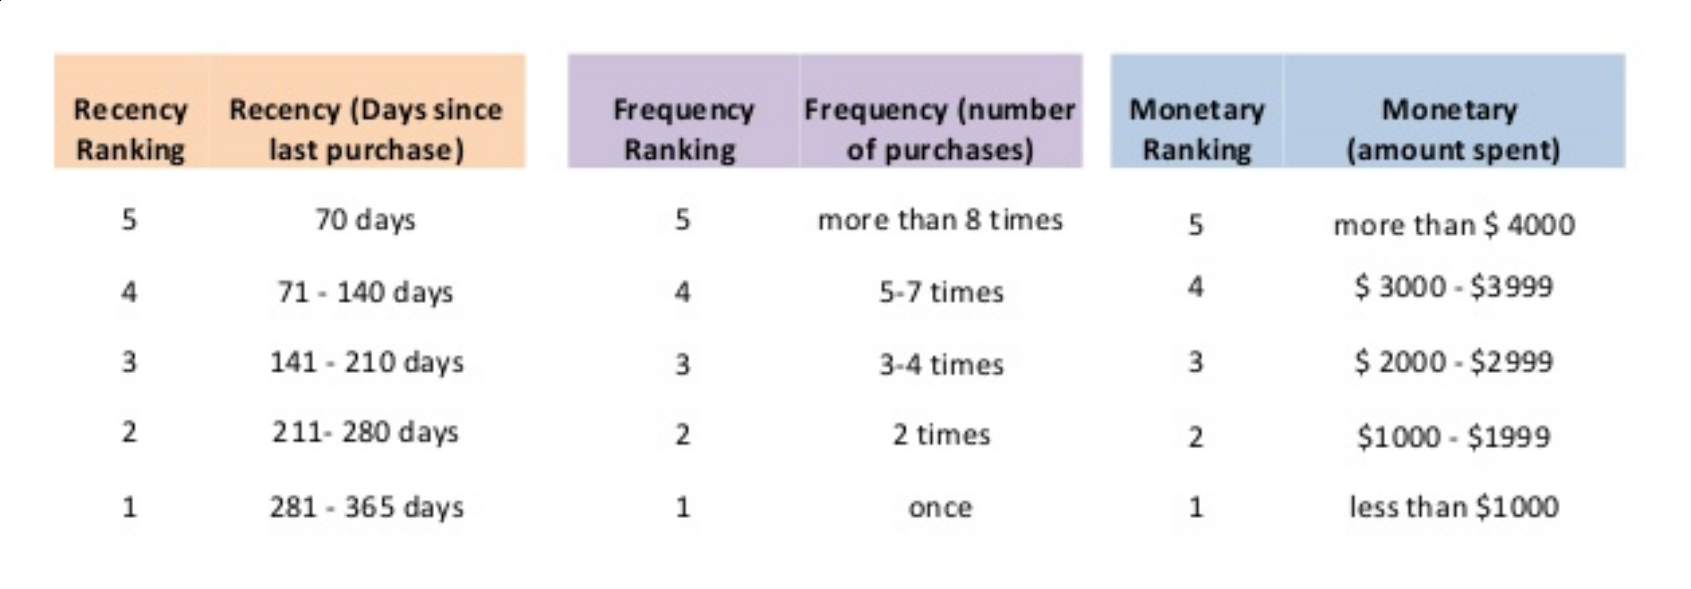
\includegraphics[scale=0.22]{../images/lec5img1}
\end{figure}

Ce modèle a donné naissance à un autre, le RFE. On remplace le M par le E, "Engagement". Ces stratégies calculent le niveau d'engagement social du client envers la marque.
